\documentclass[a4paper, 11pt]{article}

% Nécessaire
\usepackage[french]{babel}
\usepackage[utf8]{inputenc}
\usepackage[T1]{fontenc}
\usepackage{lmodern}
\usepackage{amsmath, amsthm}
\usepackage{amsfonts,amssymb}

% Marge
\usepackage{geometry}
\geometry{margin={2.2cm ,2cm}}

% Figures, graphiques
\usepackage{graphicx}
\usepackage{epsfig}
\usepackage{caption}

% Surlignage
\usepackage{alltt}

\usepackage{xcolor}
\usepackage{soul}
\usepackage{color}
\usepackage{colortbl}

% Indicatrice
\usepackage{dsfont}

\usepackage{multirow}
\usepackage{eurosym}
\usepackage{extarrows}


% Titre
\title{Changements effectués et impacts sur le modèle}
\author{}
\date{}



\begin{document}
\maketitle

Ce document présente les divers apports au modèle et leurs effets sur celui-ci.

\section{Référence}

Comme résultat de référence, on prendra le résultat donné par le modèle qui prend en entrée la dynamique $I_t^2$ avec les paramètres calibrés par NSGA-II qui prend comme critères l'ajustement sur les trois sous-blocs.

Ce résultat nous servira donc à apprécier les changements qui seront effectués

\begin{figure}[h]
 \centering
 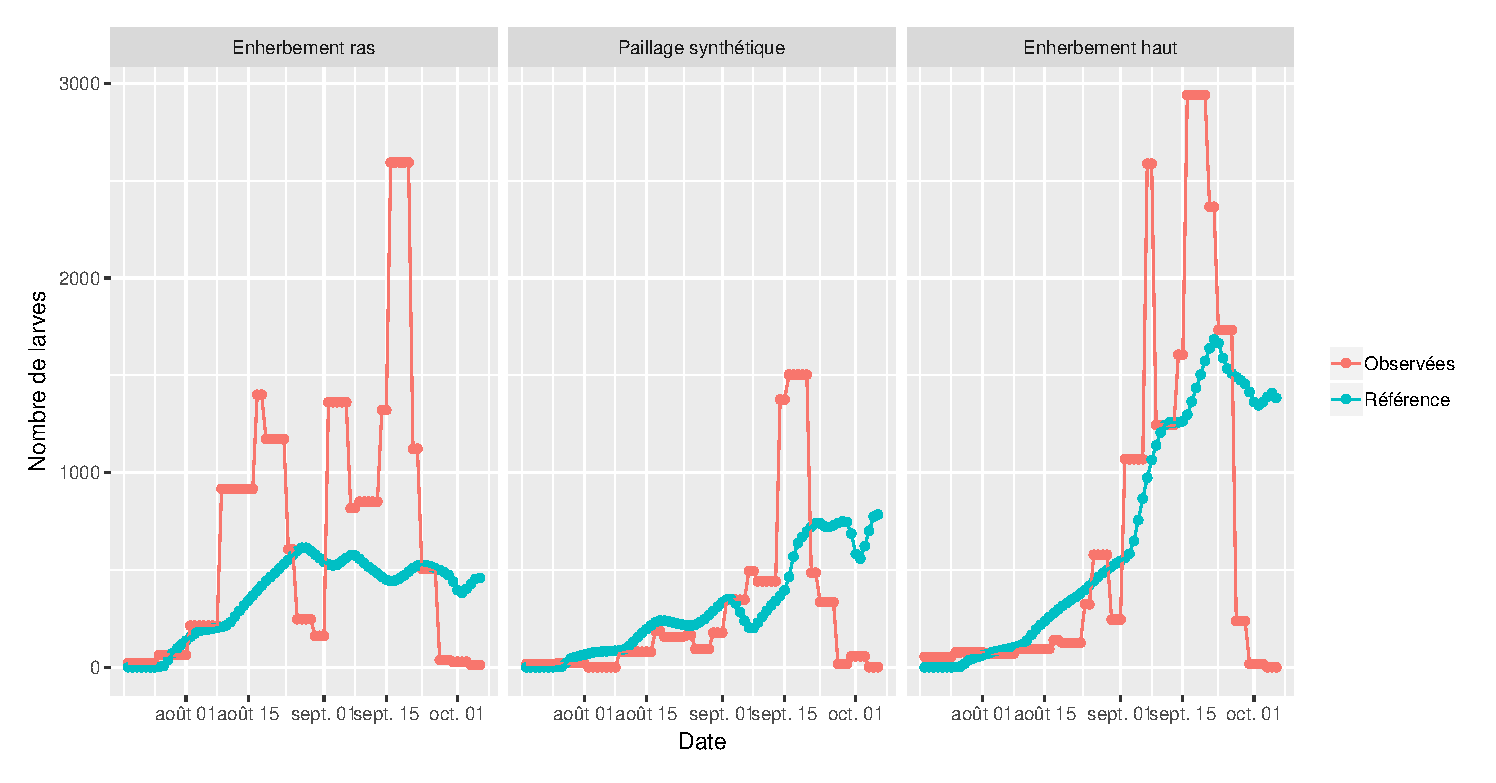
\epsfig{file = plots/ref.eps, scale = 0.65}
\end{figure}

\newpage
\section{Rajout des critères de nombres de larves totaux à NSGA-II}

La première tentative fut de rajouter à NSGA-II trois critères supplémentaires correspondant aux nombre total de larves pour chacun des trois sous-blocs.

\begin{figure}[h]
 \centering
 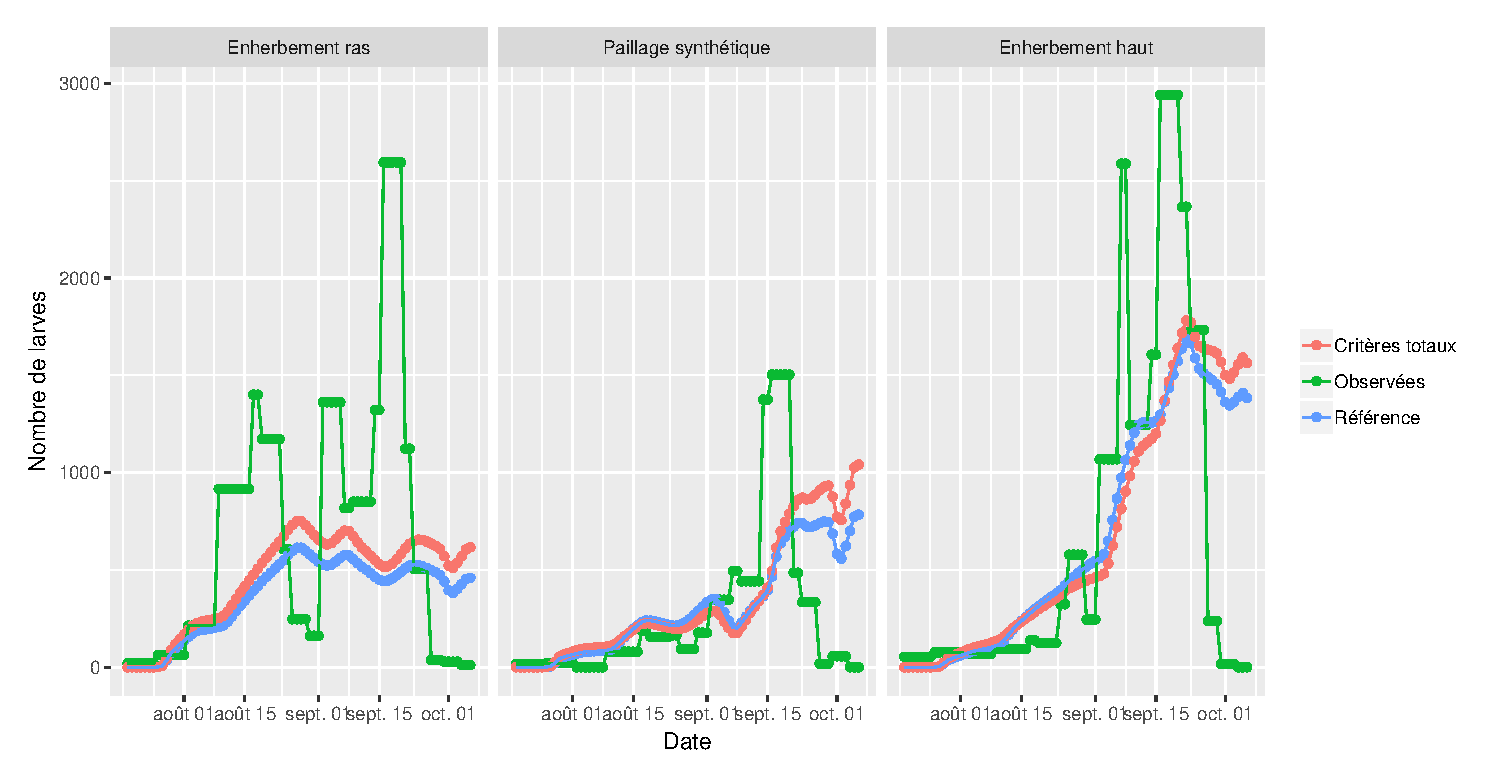
\epsfig{file = plots/nsga6.eps, scale = 0.65}
\end{figure}


\newpage
\section{Inflorescences attractives}

Il a aussi été essayé de remplacer les inflorescences vivantes $I_t^2$ par les inflorescences attractives $I_t^{a,1}$ et $I_t^{a,s}$.

Avec $I_t^{a, 1}$ : 

\begin{figure}[h]
 \centering
 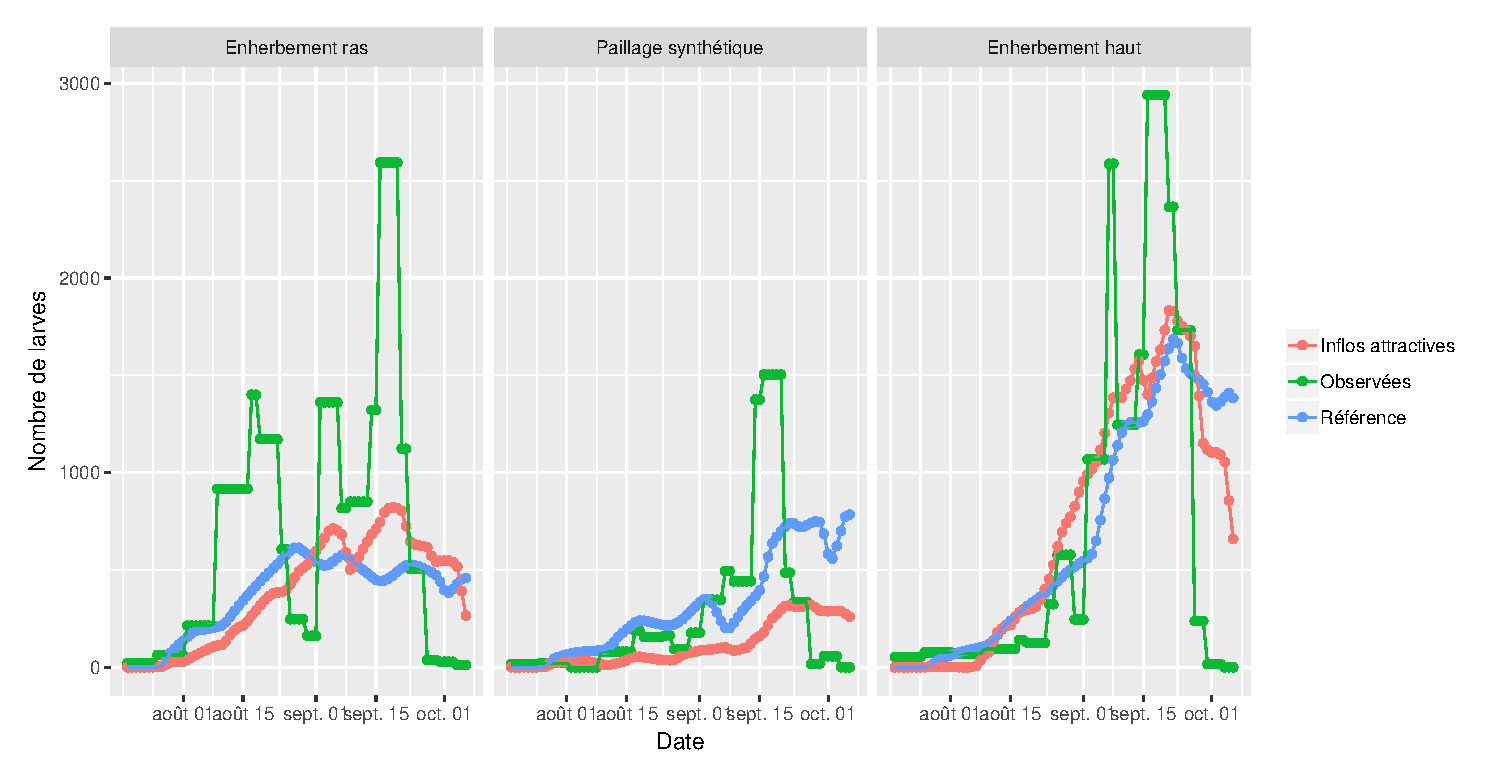
\epsfig{file = plots/la1.eps, scale = 0.65}
\end{figure}

Avec $I_t^{a,s}$ : 

\begin{figure}[h]
 \centering
 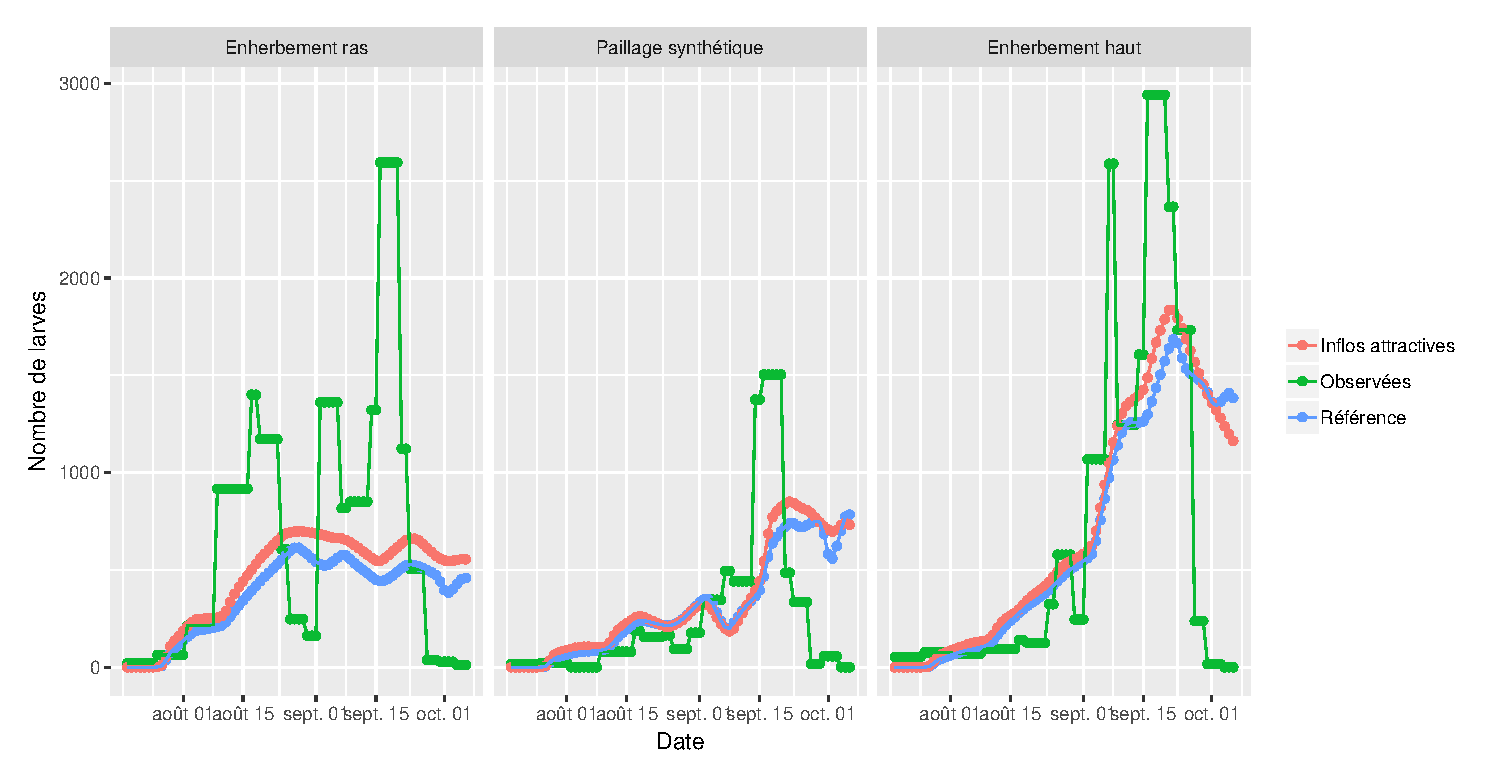
\epsfig{file = plots/las.eps, scale = 0.65}
\end{figure}

\newpage
\section{Étalement de la durée de larvation}

On aussi essayé de répartir la durée de larvation entre 7 et 12 jours après la ponte.

Avec une répartition uniforme sur $\{7, 8,9,10,11,12\}$ :
\begin{figure}[h]
 \centering
 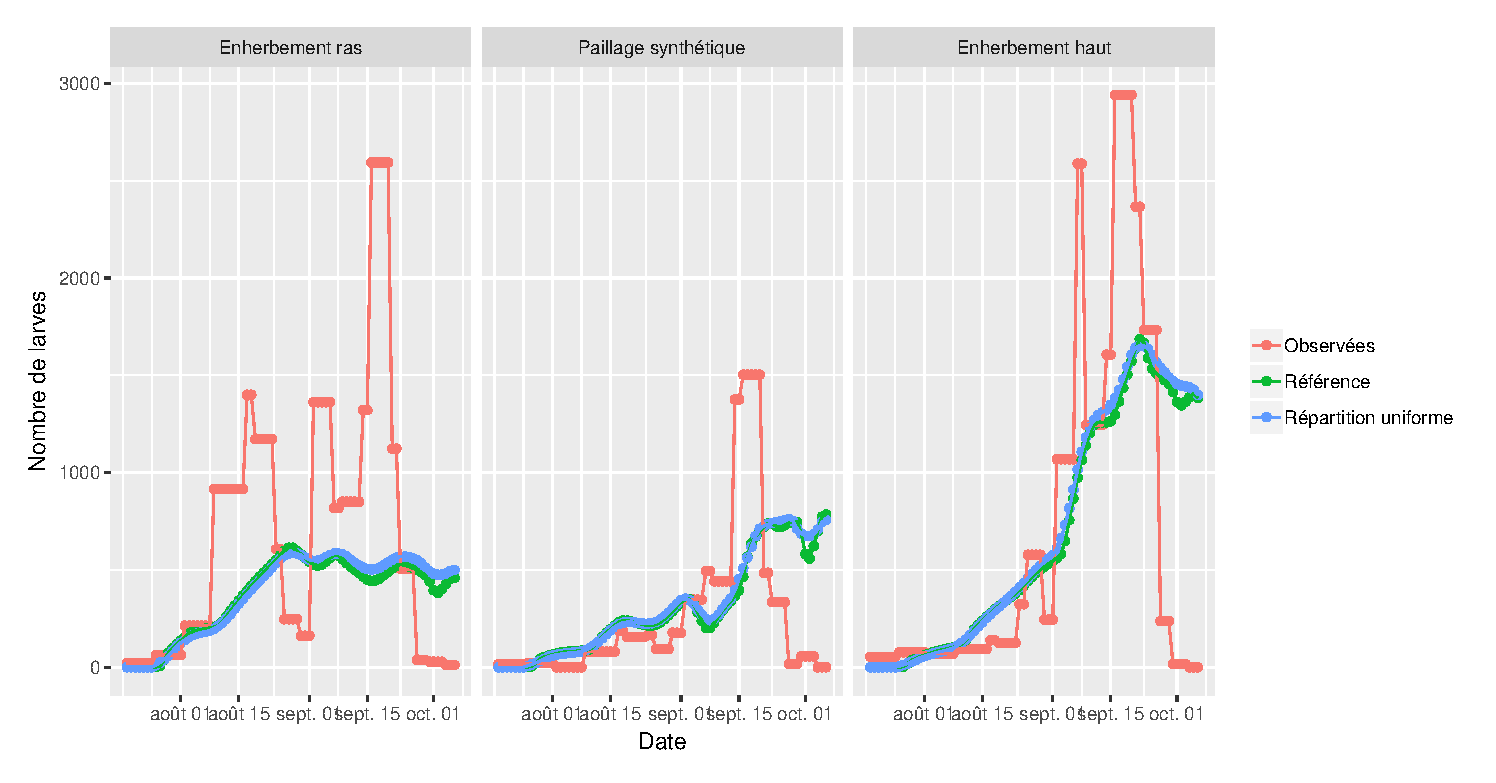
\epsfig{file = plots/luni.eps, scale = 0.65}
\end{figure}

Avec la répartition suivante \begin{center}
\begin{tabular}{cccccc}
Jour 7 & Jour 8 & Jour 9 & Jour 10 & Jour 11 & Jour 12\\
0.025 & 0.075 & 0.4 & 0.4 & 0.075 & 0.025
                           \end{tabular}
                           \end{center}

\begin{figure}[h]
 \centering
 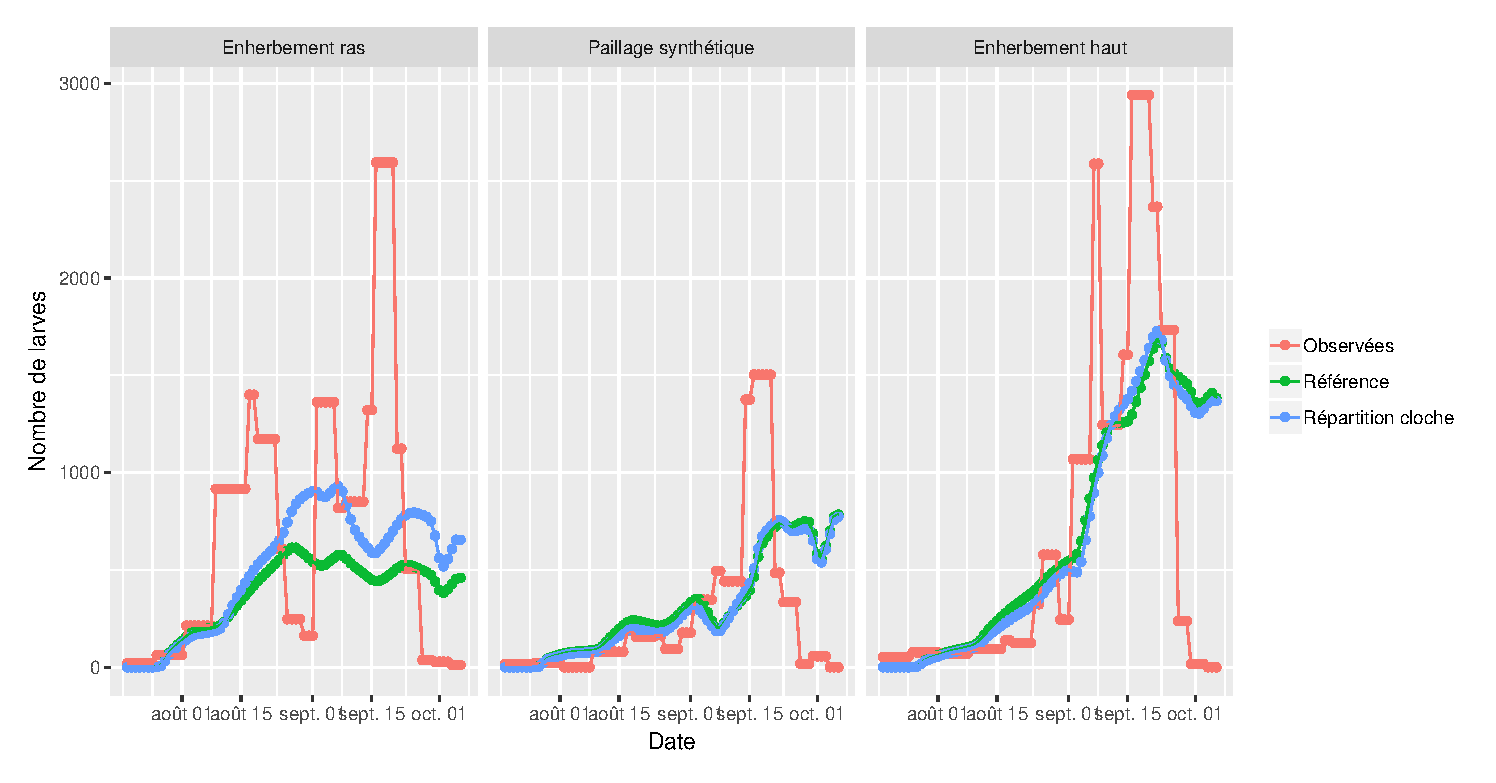
\epsfig{file = plots/lclo.eps, scale = 0.65}
\end{figure}


\newpage
\section{Calibration de $\Delta_t$}

En ne rentrant que le nombre de débourrements quotidiens simulés $B_t^s$ et en calculant les inflorescences attractives où le $\Delta_t$ est à calibrer. Le $\Delta_t$ ainsi trouvé est 11.99.

\begin{figure}[h]
 \centering
 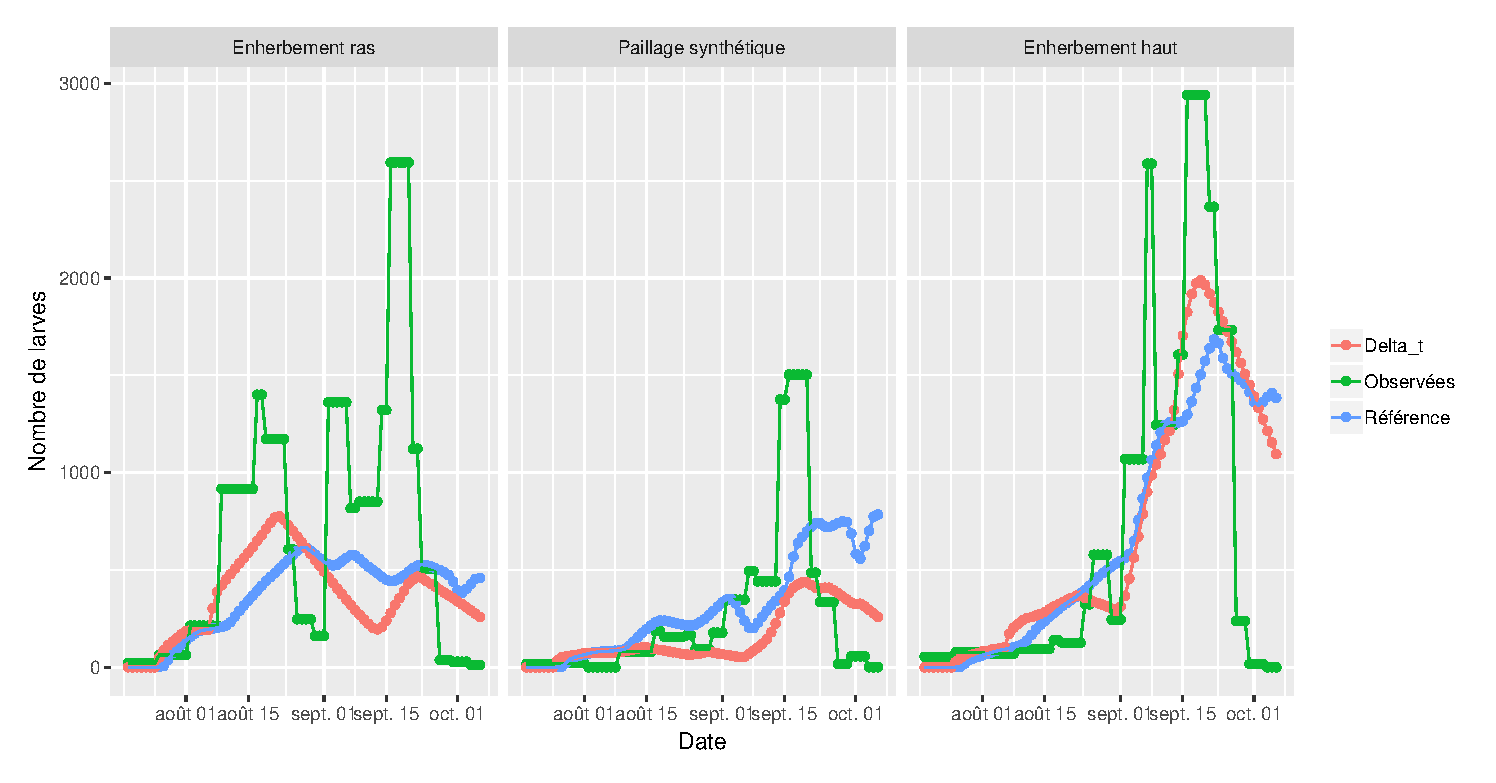
\epsfig{file = plots/deltat.eps, scale = 0.65}
\end{figure}




\newpage
\section{Toutes les modifications}

En mélangeant plusieurs critères précédents.

Ici, critères de larves totaux, répartition durée larvation en cloche, $I_t^{c,1}$

\begin{figure}[h]
 \centering
 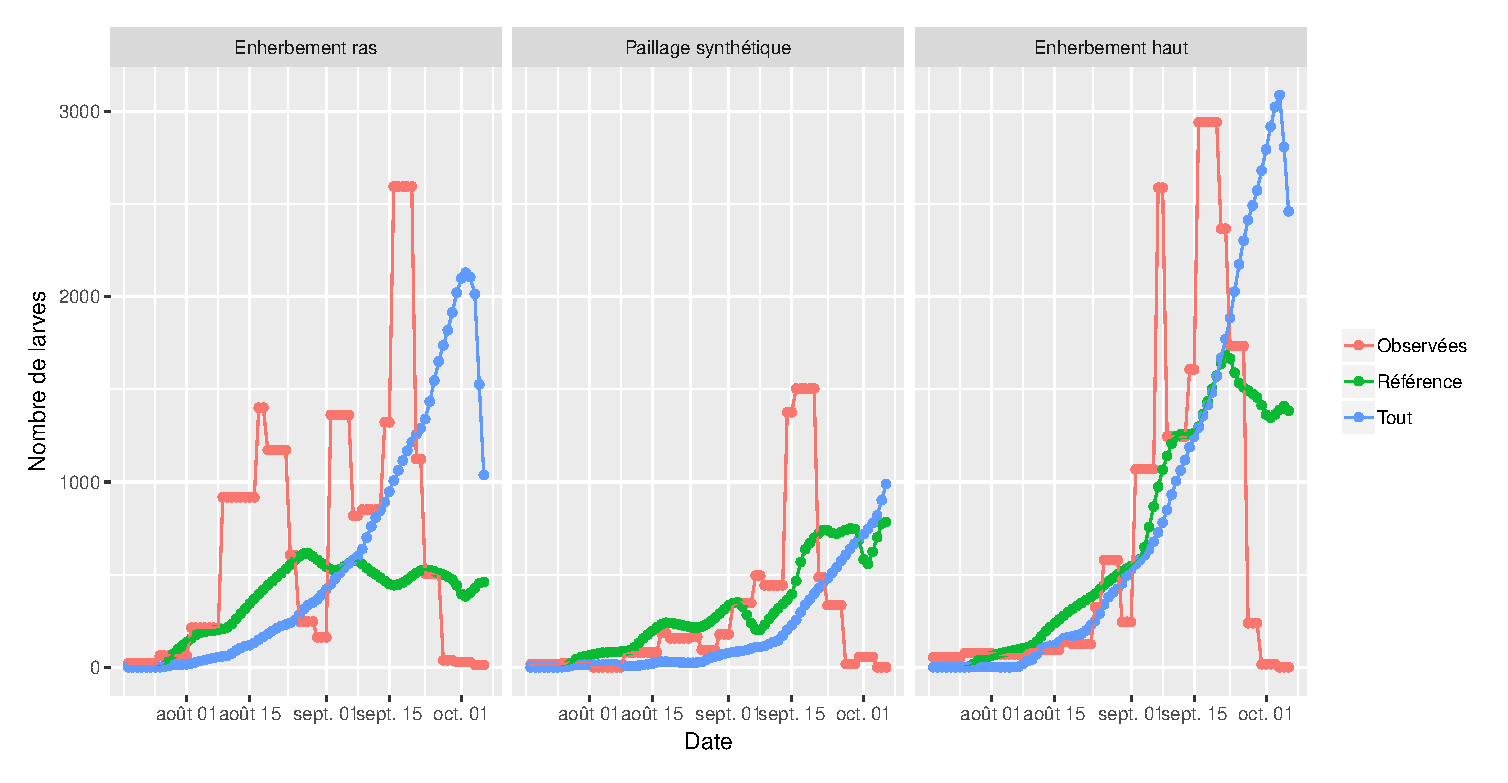
\epsfig{file = plots/ltout.eps, scale = 0.65}
\end{figure}

Ici, critères de larves totaux, répartition durée larvation en cloche, calibration de $\Delta_t$

\begin{figure}[h]
 \centering
 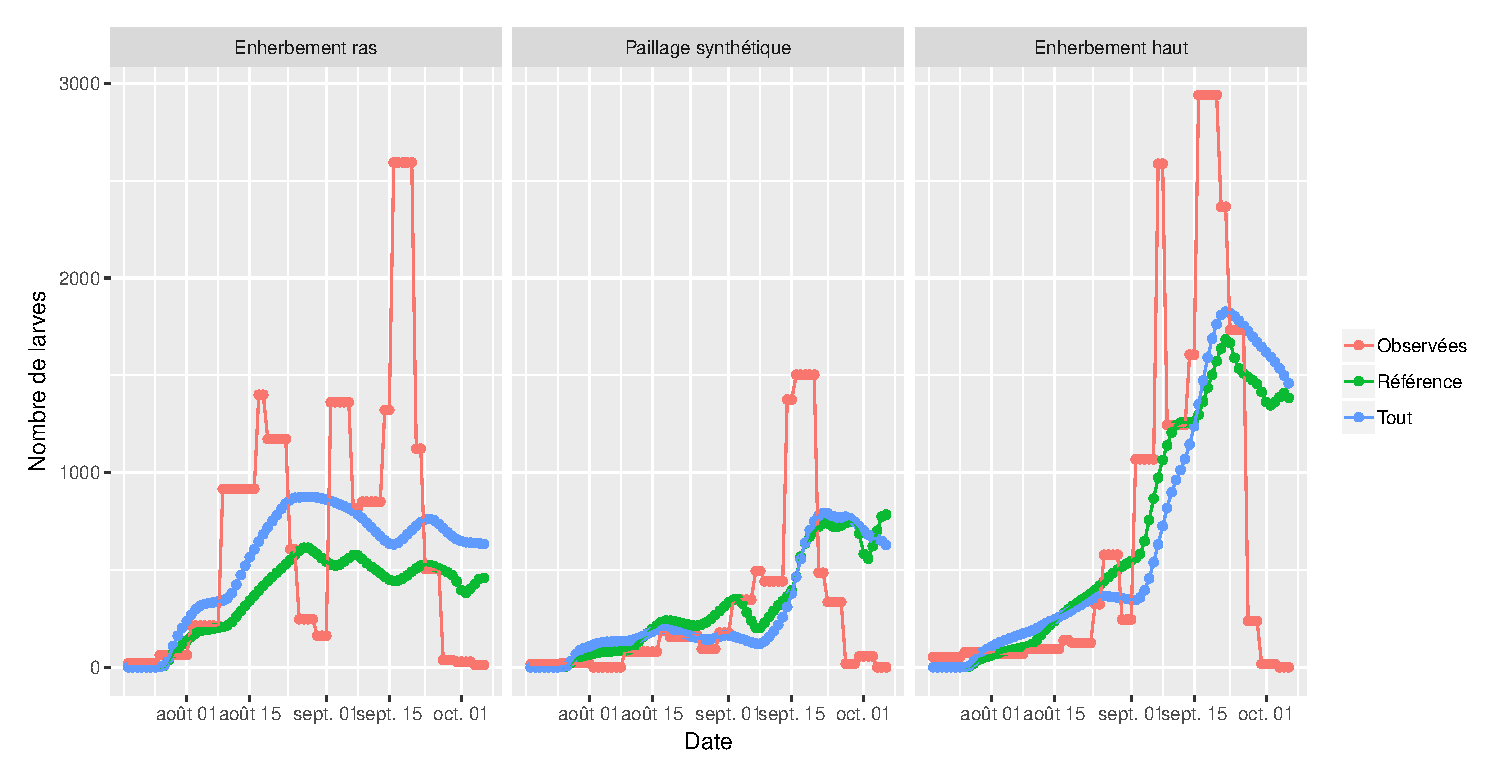
\epsfig{file = plots/ltout2.eps, scale = 0.65}
\end{figure}

\end{document}
